%----------------%
% antigo template-TESTES.tex
%----------------%

%% abtex2-modelo-trabalho-academico.tex, v-1.9 laurocesar
%% Copyright 2012-2013 by abnTeX2 group at http://abntex2.googlecode.com/ 
%%
%% This work may be distributed and/or modified under the
%% conditions of the LaTeX Project Public License, either version 1.3
%% of this license or (at your option) any later version.
%% The latest version of this license is in
%%   http://www.latex-project.org/lppl.txt
%% and version 1.3 or later is part of all distributions of LaTeX
%% version 2005/12/01 or later.
%%
%% This work has the LPPL maintenance status `maintained'.
%% 
%% The Current Maintainer of this work is the abnTeX2 team, led
%% by Lauro César Araujo. Further information are available on 
%% http://abntex2.googlecode.com/
%%
%% This work consists of the files abntex2-modelo-trabalho-academico.tex,
%% abntex2-modelo-include-comandos and abntex2-modelo-references.bib
%%

% ------------------------------------------------------------------------
% ------------------------------------------------------------------------
% abnTeX2: Modelo de Trabalho Academico (tese de doutorado, dissertacao de
% mestrado e trabalhos monograficos em geral) em conformidade com 
% ABNT NBR 14724:2011: Informacao e documentacao - Trabalhos academicos -
% Apresentacao
% ------------------------------------------------------------------------
% ------------------------------------------------------------------------

\documentclass[
	% -- opções da classe memoir --
	12pt,				% tamanho da fonte
	openany,			% capítulos começam em pág ímpar (insere página vazia caso preciso) - openright ou openany
	oneside,			% para impressão em verso e anverso. Oposto a oneside
	a4paper,			% tamanho do papel. 
	% -- opções da classe abntex2 --
	%chapter=TITLE,		% títulos de capítulos convertidos em letras maiúsculas
	%section=TITLE,		% títulos de seções convertidos em letras maiúsculas
	%subsection=TITLE,	% títulos de subseções convertidos em letras maiúsculas
	%subsubsection=TITLE,% títulos de subsubseções convertidos em letras maiúsculas
	% -- opções do pacote babel --
	english,			% idioma adicional para hifenização
	french,				% idioma adicional para hifenização
	spanish,			% idioma adicional para hifenização
	brazil				% o último idioma é o principal do documento
	]{abntex2}

% ---
% PACOTES
% ---

% ---
% Pacotes fundamentais 
% ---
\usepackage{lmodern}			% Usa a fonte Latin Modern			
\usepackage[T1]{fontenc}		% Selecao de codigos de fonte.
\usepackage[utf8]{inputenc}		% Codificacao do documento (conversão automática dos acentos)
\usepackage{lastpage}			% Usado pela Ficha catalográfica
\usepackage{indentfirst}		% Indenta o primeiro parágrafo de cada seção.
\usepackage{color}				% Controle das cores
\usepackage{graphicx}			% Inclusão de gráficos
\usepackage[export]{adjustbox}  % Permite usar a opção frame ou fbox, para criar margem nas figuras
\usepackage[singlelinecheck=false]{caption} % Manter caption à esquerda
\usepackage{microtype} 			% para melhorias de justificação
\usepackage{rotating}           %rotação de texto
%\usepackage[landscape]{geometry}% http://ctan.org/pkg/geometry
\usepackage{array}              % http://ctan.org/pkg/array
\usepackage[table,xcdraw]{xcolor}
\usepackage[printonlyused]{acronimos-extendido}
\usepackage{textcase}
\usepackage{caption}
\usepackage{subcaption}
\usepackage{multirow}
\usepackage{booktabs}
\usepackage{pifont}
% Utilizado para inserir arquivos PDF no documento
\RequirePackage{pdflscape}
\RequirePackage{pdfpages}
% EXEMPLO: \includepdf[pages=1-2,scale=1]{1st_texts/lista_quadros.pdf}

% Utilizado para inserir quadros no documento
%\usepackage{trivfloat}
%\trivfloat{quadro}
% Substituído comando acima por entradas no arquivo "abntex2.cls". Referência de comandos tiradas de: https://github.com/abntex/abntex2/wiki/HowToCriarNovoAmbienteListing





% ---

% Comando para girar texto da tabela em 90 graus
\newcommand*\giranov{\rotatebox{90}}	

% Comando para inserir um texto sobrescrito
\newcommand{\ts}{\textsuperscript}

% Comandos para auxiliar na revisão:
%\usepackage{cancel,soul,ulem}
\usepackage[normalem]{ulem}
\usepackage{color,pgf}
\usepackage{verbatim}

\newcommand{\excluir}[2]{
\textcolor{red}{\textbf{#1: }\sout{#2}}
}

\newcommand{\incluir}[2]{
\textcolor{green}{\textbf{#1: }\textbf{#2}}
}

% Pacote para inserir TODO, para correção
\usepackage[colorinlistoftodos,prependcaption,textsize=tiny]{todonotes}


% ---
% Pacotes de citações
% ---
% Citações padrão ABNT (algumas opções):
% alf: lista autores em ordem alfabética
% abnt-emphasize=bf: coloca o título das referências em negrito. Se tirar, fica em itálico.

% \usepackage[alf,myoptions]{abntex2cite} % Citações padrão ABNT
\usepackage[alf,abnt-etal-list=0,abnt-etal-cite=3,abnt-repeated-author-omit=yes,abnt-doi=expand,abnt-emphasize=bf]{abntex2cite}	



% Pacote de Formatação da Univali
\usepackage{univali_custom}


% ---
% Informações de dados para CAPA e FOLHA DE ROSTO
% ---
\titulo{GERENCIAMENTO DE FLUXO DE POTÊNCIA EM USINAS FOTOVOLTAICAS CONSIDERANDO O ARMAZENAMENTO DE ENERGIA EM BATERIAS}
%\subtitulo{subtítulo se houver}
\autor{Camila de Souza}
\local{Itajaí (SC)}
\mes{Abril}
\ano{2024}
\orientador{Maurício de Campos, Dr.}
%\coorientador{Coorientador}
\instituicao{UNIVERSIDADE DO VALE DO ITAJAÍ\par
PRÓ-REITORIA DE PÓS-GRADUAÇÃO,\\ 
PESQUISA, EXTENSÃO E CULTURA\par
PROGRAMA DE MESTRADO ACADÊMICO EM\\ 
COMPUTAÇÃO APLICADA}

\tipotrabalho{Qualificação de Dissertação (Mestrado)}
% O preambulo deve conter o tipo do trabalho, o objetivo, 
% o nome da instituição e a área de concentração 
\preambulo{Dissertação apresentada como requisito parcial à obtenção do grau de Mestre em Computação Aplicada.}
% ---

% ---
% Informações para Resumo e Abstract
% ---
\linhadepesquisa{Sistemas Inteligentes e Educacionais}
\researchline{Intelligent and Educational Systems}
%\numpaginas{175}
\palavraschave{palavra 1, palavra 2, palavra 3.}
\keywords{word 1, word 2, word 3.}
\englishmonth{April}
\titleenglish{Mobile Identity for Brazilian Government}
\subtitleenglish{A User-Centric Solution for e-Government}
% ---


% ---
% Configurações de aparência do PDF final

% informações do PDF
\makeatletter
\hypersetup{
     	%pagebackref=true,
		pdftitle={\@title}, 
		pdfauthor={\@author},
    	pdfsubject={\imprimirpreambulo},
	    pdfcreator={LaTeX with abnTeX2},
		pdfkeywords={trabalho acadêmico}, 
		colorlinks=true,       		% false: boxed links; true: colored links
    	linkcolor=black,          	% color of internal links
    	citecolor=black,        		% color of links to bibliography
    	filecolor=black,      		% color of file links
		urlcolor=black,
		bookmarksdepth=4
}
\makeatother
% --- 

% ---
% compila o indice
% ---
\makeindex

% ----
% Início do documento
% ----
\begin{document}

% Retira espaço extra obsoleto entre as frases.
\frenchspacing 


% ----------------------------------------------------------
% ELEMENTOS PRÉ-TEXTUAIS
% ----------------------------------------------------------
% \pretextual

% ---
% Capa
% ---
\imprimircapa
% ---

% ---
% Folha de rosto
% (o * indica que haverá a ficha bibliográfica)
% ---
\imprimirfolhaderosto*
% ---

% ---
% Inserir a ficha bibliografica
% ---
%% Isto é um exemplo de Ficha Catalográfica, ou ``Dados internacionais de
% catalogação-na-publicação''. Você pode utilizar este modelo como referência. 
% Porém, provavelmente a biblioteca da sua universidade lhe fornecerá um PDF
% com a ficha catalográfica definitiva após a defesa do trabalho. Quando estiver
% com o documento, salve-o como PDF no diretório do seu projeto e substitua todo
% o conteúdo de implementação deste arquivo pelo comando abaixo:
%
% \begin{fichacatalografica}
%     \includepdf{fig_ficha_catalografica.pdf}
% \end{fichacatalografica}
\begin{fichacatalografica}
	\vspace*{\fill}					% Posição vertical
	\hrule							% Linha horizontal
	\begin{center}					% Minipage Centralizado
	\begin{minipage}[c]{12.5cm}		% Largura
	
	\imprimirautor
	
	\hspace{0.5cm} \imprimirtitulo  / \imprimirautor. --
	\imprimirlocal, \imprimirdata-
	
	\hspace{0.5cm} \pageref{LastPage} p. : il. (algumas color.) ; 30 cm.\\
	
	\hspace{0.5cm} \imprimirorientadorRotulo~\imprimirorientador\\
	
	\hspace{0.5cm}
	\parbox[t]{\textwidth}{\imprimirtipotrabalho~--~\imprimirinstituicao,
	\imprimirdata.}\\
	
	\hspace{0.5cm}
		1. Palavra-chave1.
		2. Palavra-chave2.
		I. Orientador.
		II. Universidade xxx.
		III. Faculdade de xxx.
		IV. Título\\ 			
	
	\hspace{8.75cm} CDU 02:141:005.7\\
	
	\end{minipage}
	\end{center}
	\hrule
\end{fichacatalografica}
% ---
% ---

% ---
% Inserir folha de aprovação
% ---

% Isto é um exemplo de Folha de aprovação, elemento obrigatório da NBR
% 14724/2011 (seção 4.2.1.3). Você pode utilizar este modelo até a aprovação
% do trabalho. Após isso, substitua todo o conteúdo deste arquivo por uma
% imagem da página assinada pela banca com o comando abaixo:
%
% \includepdf{folhadeaprovacao_final.pdf}
%
%\begin{folhadeaprovacao}

  \begin{center}
    {\ABNTEXchapterfont\large\imprimirautor}

    \vspace*{\fill}\vspace*{\fill}
    \begin{center}
      \ABNTEXchapterfont\bfseries\Large\imprimirtitulo
    \end{center}
    \vspace*{\fill}
    
    \hspace{.45\textwidth}
    \begin{minipage}{.5\textwidth}
        \imprimirpreambulo
    \end{minipage}%
    \vspace*{\fill}
   \end{center}
        
   Trabalho aprovado. \imprimirlocal, 24 de novembro de 2012:

   \assinatura{\textbf{\imprimirorientador} \\ Orientador} 
   \assinatura{\textbf{Professor} \\ Convidado 1}
   \assinatura{\textbf{Professor} \\ Convidado 2}
   %\assinatura{\textbf{Professor} \\ Convidado 3}
   %\assinatura{\textbf{Professor} \\ Convidado 4}
      
   \begin{center}
    \vspace*{0.5cm}
    {\large\imprimirlocal}
    \par
    {\large\imprimirdata}
    \vspace*{1cm}
  \end{center}
  
\end{folhadeaprovacao}

%\begin{dedicatoria}
    \vspace*{\fill}
	\begin{flushright}
		\textit{Página opcional reservada para dedicatórias, as quais devem ser escritas em itálico, alinhadas à direita e posicionadas na base da página. Exclua esta página se não for incluir nenhuma dedicatória. Só escreva para a versão final, não fica para a qualificação!}
	\end{flushright}
\end{dedicatoria}
\begin{epigrafe}
    \vspace*{\fill}
	\begin{flushright}
		\textit{``Mensagem''}		
	\end{flushright}
\end{epigrafe}
\begin{agradecimentos}

Texto destinado aos agradecimento.. vai só na versão final, não na qualificação!

\end{agradecimentos}
% Formatação de Resumo - pg 267 do arquivo "univali_custom.sty"
\setlength{\absparsep}{14pt} 
\begin{resumo}
O Resumo é um dos componentes mais importantes do trabalho. É partir dele que o leitor irá decidir se vale a pena continuar lendo o trabalho ou não. O resumo deve ser escrito como um parágrafo único, sem utilizar referências bibliográficas e evitando ao máximo, o uso de siglas/abreviações. O resumo deve conter entre 200 e 400 palavras, sendo composto das seguintes partes (organização lógica): introdução, objetivos, justificativa, metodologia, resultados esperados ou obtidos. Esta é a seqüência lógica, não devendo ser utilizados títulos e subtítulos. Não abuse na contextualização, pois o foco deve ser nos objetivos, resultados esperados e resultados obtidos. Escreva o resumo apenas após a conclusão do trabalho. Ele deve refletir bem aquilo que foi desenvolvido.
\end{resumo}
\begin{abstract}
 \begin{otherlanguage*}{english}
 
Abstract

\end{otherlanguage*}
\end{abstract}


% ---
% inserir lista de ilustrações
% ---
\pdfbookmark[0]{\listfigurename}{lof}
\listoffigures*
% \cleardoublepage
% ---
% ---
% inserir lista de tabelas
% ---
\pdfbookmark[0]{\listtablename}{lot}
\listoftables*
% \cleardoublepage
% ---
%\includepdf[pages=1,scale=1]{1st_texts/lista_quadros.pdf}
% ---
% inserir lista de quadros
% ---
%\newpage
%\phantomsection
\pdfbookmark[0]{\listofquadrosname}{loq}
\listofquadros*
\cleardoublepage
% ---


%\begin{siglas}
\item[6LoWPAN]{\textit{IPv6 over Low Power Wireless Personal Area Networks}}
\item[ABAC]{\textit{Attribute Based Access Control}}	 
\item[AC]{Autoridade Certificadora}
\item[ACL]{\textit{Access Control List}}
\item[ACM]{\textit{Access Control Mechanism}}
\item[AES]{\textit{Advanced Encryption Standard}}
\item[API]{\textit{Application Programming Interface}}
\item[AS]{\textit{Authorized Server}}
\item[BPEL]{\textit{Business Process Execution Language}}
\item[DAC]{\textit{Discretionary Access Control}}	
\item[DoS]{\textit{Denial of Service}}	
\item[DTLS]{\textit{Datagram Transport Layer Security}}
\item[EAP]{\textit{Extensible Authentication Protocol}}	
\item[ECC]{\textit{Elliptic Curve Cryptography}}
\item[ECCDH]{\textit{ECC Diffie-Hellman}}
\item[ECP]{\textit{Enhanced Client or Proxy}}
\item[EnHANTs]{\textit{Energy-Harvesting Active Networked Tags}}
\item[GID]{Gestão de Identidades Digitais}
\item[HTML]{\textit{Hypertext Markup Language}}
\item[HTTP]{\textit{Hypertext Transfer Protocol}}
\item[IAA]{Infraestrutura de Autenticação e Autorização}
\item[IdM]{\textit{Identity Management}}
\item[IdP]{\textit{Identity Provider}}
\item[IoT]{\textit{Internet of Things}}
\item[IP]{\textit{Internet Protocol}}
\item[IPv4]{\textit{Internet Protocol version 4}}
\item[IPv6]{\textit{Internet Protocol version 6}}
\item[JSON]{\textit{JavaScript Object Notation}}
\item[KDC]{\textit{Key Distribution Center}}
\item[LDAP]{\textit{Lightweight Directory Access Protocol}}	
\item[M2M]{\textit{Machine to Machine}}
\item[MAC]{\textit{Mandatory Access Control}}
\item[MITM]{\textit{Man-In-The-Middle}}
\item[NFC]{\textit{Near-Field Communication}}
\item[PAP]{\textit{Policy Administration Point}}
\item[PBAC]{\textit{Policy-Based Access Control}}
\item[PDP]{\textit{Policy Decision Point}}
\item[PEP]{\textit{Policy Enforcement Point}}
\item[PIP]{\textit{Policy Information Point}}
\item[RAM]{\textit{Random Access Memory}}
\item[RBAC]{\textit{Role Based Access Control}}
\item[REST]{\textit{REpresentational State Transfer}}
\item[RFID]{\textit{Radio-Frequency IDentification}}
\item[ROA]{\textit{Resource Oriented Architecture}}
\item[ROM]{\textit{Read-only Memory}}
\item[RSN]{\textit{RFID Sensor Network}}
\item[RSSF]{Redes de Sensores Sem Fio}
\item[SGML]{\textit{Standard Generalized Markup Language}}
\item[SAML]{\textit{Security Assertion Markup Language}}
\item[SP]{\textit{Service Provider}}
\item[SSO]{\textit{Single Sign-On}}
\item[TLS]{\textit{Transport Layer Security}}
\item[TPM]{\textit{Trusted Platform Module}}
\item[UDDI]{\textit{Universal Description, Discovery and Integration}}
\item[URI]{\textit{Uniform Resource Identifier}}
\item[URL]{\textit{Uniform Resource Locator}}
\item[WoT]{\textit{Web of Things}}
\item[WABAC]{\textit{Workflow-oriented Attributed Based Access Control}}
\item[WSAN]{\textit{Wireless Sensor and Actuator Network}}
\item[WSDL]{\textit{Web Services Description Language}}
\item[WSN]{\textit{Wireless Sensor Network}}
\item[XML]{\textit{eXtensible Markup Language}}
\item[XACML]{\textit{eXtensible Access Control Markup Language}}	
\end{siglas}
%% ---
% inserir lista de símbolos
% ---
\begin{simbolos}
  \item[$ \Gamma $] Letra grega Gama
  \item[$ \Lambda $] Lambda
  \item[$ \zeta $] Letra grega minúscula zeta
  \item[$ \in $] Pertence
\end{simbolos}

% ---

%% Como usar o pacote acronym


% Na primeira vez que for citado o acronimo, o nome completo 
% irá aparecer seguido do acronimo entre parênteses. Na 
% proxima vez somente o acronimo irá aparecer. Se usou a 
% opção footnote no pacote, entao o nome por extenso irá 
% aparecer no rodapé \ac{acronimo}


% Para aparecer com nome completo + acronimo
% \acf{acronimo}

% Para aparecer somente o acronimo
% \acs{acronimo}

% Nome por extenso somente, sem o acronimo
% \acl{acronimo}

% igual o \ac mas deixando no plural com S (ingles)
% \acp{acronimo}

% \acfp{acronimo}

% \acsp{acronimo}

% \aclp{acronimo}

%% ATENCAO
% Criei o comando \acfe{}, resultando em: Extenso -- ACRO

\chapter*{Lista de Abreviaturas}%
% \addcontentsline{toc}{chapter}{Lista de abreviaturas}
\markboth{Lista de abreviaturas}{}


\begin{acronym}







%A
\acro{AA}{\textit{Attribute Authority}}
\acro{ABAC}{\textit{Attribute-Based Access Control}}
\acro{AC}{Autoridade Certificadora}
\acro{AD}{\textit{Active Directory}}
\acro{AES}{\textit{Advanced Encryption Standard}}
\acro{AP}{\textit{Attribute Provider}}
\acro{APIs}{\textit{Application Programming Interfaces}}
\acro{APP}{\textit{Application}}
\acro{ARC}{\textit{Advanced Resource Connector}}
\acro{AS}{\textit{Attribute Service}}
\acro{ASM}{\textit{Authenticator Abstraction Layer}}
\acro{ASP}{\textit{Application Service Provider}}
\acro{ATN}{\textit{Automated Trust Negotiation}}
%B
\acro{BLE}{\textit{Bluetooth Low Energy}}
%C
\acro{CA}{\textit{Certificate Authority}}
\acro{CN}{\textit{Collaborative Networks}}
\acro{CNH}{Carteira Nacional de Habilitação}
\acro{CNPJ}{Cadastro Nacional de Pessoa Jurídica}
\acro{CPF}{Cadastro de Pessoa Física}
\acro{CS}{\textit{Consent Service}}
\acro{CSR}{\textit{Certificate Signing Request}}
\acro{CPU}{\textit{Central Processing Unit}}
%D
\acro{DFN}{\textit{Deutsches Forschungsnetz}}
\acro{DN}{\textit{Distinguised Name}}
\acro{DS}{\textit{Discovery Service}}
\acro{DVO}{\textit{Dynamic Virtual Organization}}
%E
\acro{e-CPF}{Cadastro de Pessoal Física Eletrônico}
\acro{e-CNPJ}{Cadastro Nacional de Pessoa Jurídica Eletrônico}
\acro{e-Gov}{\textit{Electronic Government}}
\acro{e-PING}{Padrões de Interoperabilidade em Governo Eletrônico}
\acro{eID}{\textit{Electronic Identity}}
\acro{eIDMS}{\textit{electronic Identity Management System}}
\acro{EGDI}{\textit{e-Government Development Index}}
\acro{ePWG}{Padrões Web para Governo Eletrônico}
\acro{ETSI}{\textit{European Telecommunications Standards Institute}}
%F
\acro{FIDO}{\textit{Fast IDentity Online}}
\acro{FIM}{\textit{Federated Identity Management}}
\acro{FO}{\textit{Federation Operator}}
%G
\acro{G2C}{Governo para Cidadão}
\acro{G2E}{\textit{Government to Employees}}
\acro{G2G}{Governo para Governo}
\acro{GId}{Gestão de Identidade}
\acro{GSI}{\textit{Grid Security Infrastructure}}
\acro{GTTI}{Grupo de Trabalho Interministerial}
%H
\acro{HCE}{\textit{Host-based Card Emulation}}
\acro{HCI}{\textit{Human Capital Index}}
\acro{HPC}{\textit{High Performance Computing}}
\acro{HSM}{\textit{Hardware Security Module}}
\acro{HTTP}{\textit{Hypertext Transfer Protocol}}
%I
\acro{IAA}{\textit{Identity, Authentication, Authorization}}
\acro{IAF}{\textit{Identity Assurance Framework}}
\acro{IAM}{\textit{Identity and Access Management}}
\acro{IBAC}{\textit{Identity-Based Access Control}}
\acro{ICFF}{\textit{Intercloud Federation Framework}}
\acro{ICP}{Infraestrutura de Chave Pública}
\acro{Id}{\textit{Identity}}
\acro{ID}{Identificador}
\acro{IDE}{\textit{Integrated Development Environment}}
\acro{IdM}{\textit{Identity Management System}}
\acro{IdP}{\textit{Identity Provider}}
\acro{IGF}{\textit{Identity Governance Framework}}
\acro{IMSI}{\textit{International Mobile Subscriber Identity}}
\acro{IP}{\textit{Internet Protocol}}
\acro{IRPF}{Imposto de Renda de Pessoal Física}
%J
\acro{JSON}{\textit{JavaScript Object Notation}}
%K
%L
\acro{LDAP}{\textit{Lightweight Directory Access Protocol}}
\acro{LSDMA}{\textit{Large Scale Data Management}}
%M
\acro{MITM}{\textit{Man-in-The-Middle}}
\acro{myVOCS}{\textit{my Virtual Organization Collaboration System}}
%N
\acro{NFC}{\textit{Near Field Communication}}
\acro{NREN}{\textit{National Research Education Networks}}
%O
\acro{OASIS}{\textit{Organization for the Advancement of Structured Information Standards}}
\acro{OCSP}{\textit{Online Certificate Status Protocol}}
\acro{ONG}{Organizações Não Governamentais}
\acro{OSI}{\textit{Online Service Index}}
\acro{OTP}{\textit{One-time Password}}
\acro{OV}{Organização Virtual}
%P
\acro{PaaS}{\textit{Plataform-as-a-Service}}
\acro{PAPI}{\textit{Point of Access to Providers of Information}}
\acro{PC}{\textit{Professional Communities}}
\acro{PDP}{\textit{Policy Decision Point}}
\acro{PEP}{\textit{Policy Enforcement Point}}
\acro{PERMIS}{\textit{Privilege Managerment Infrastructure}}
\acro{PKI}{\textit{Public Key Infrastructure}}
\acro{PIC}{\textit{Personal Identification Code}}
\acro{PIN}{\textit{Personal Identification Number}}
\acro{PoA}{\textit{Point of Authentication}}
\acro{PPP}{Parceria Público-Privada}
\acro{PVC}{\textit{Professional Virtual Communities}}
%Q
%R
\acro{RA}{\textit{Registration Authority}}
\acro{RBAC}{\textit{Role-Based Access Control}}
\acro{RCN}{Registro Civil Nacional}
\acro{REE}{\textit{Rich Execution Environment}}
\acro{RIC}{Registro de Identidade Civil}
\acro{RG}{Registro Geral}
\acro{RP}{\textit{Relying Party}}
\acro{RSA}{}
\acro{RSL}{Revisão Sistemática da Literatura}
%S
\acro{SAML}{\textit{Security Assertion Markup Language}}
\acro{SAT}{\textit{SIM Application Toolkit}}
\acro{SB}{\textit{Service Broker}}
\acro{SCE}{\textit{Secure Collaborative Environment}}
\acro{SE}{\textit{Secure Element}}
\acro{SEM}{\textit{Scanning Electron Microscope}}
\acro{SGId}{Sistema de Gestão de Identidade}
\acro{SIG}{\textit{Special Interest Group}}
\acro{SIM}{\textit{Subscriber Identification Module}}
\acro{SISP}{Sistema de Administração dos Recursos de Tecnologia da Informação}
\acro{SLCS}{\textit{Short Lived Credential Service}}
\acro{SMC}{\textit{Secure Memory Card}}
\acro{SO}{Sistema Operacional}
\acro{SOAP}{\textit{Simple Object Access Protocol}}
\acro{SoC}{\textit{System on Chip}}
\acro{SP}{\textit{Service Provider}}
\acro{SSL}{\textit{Secure Sockets Layer}}
\acro{SSO}{\textit{Single Sign-On}}
\acro{SSTC}{\textit{Security Services Technical Committee}}
\acro{STORK}{\textit{Secure idenTity acrOss boRders linKed}}
%T
\acro{TAL}{\textit{Trust Anchor List}}
\acro{TEE}{\textit{Trusted Execution Environment}}
\acro{TIC}{Tecnologia da Informação e Comunicação}
\acro{TII}{\textit{Telecommunication Infrastructure Index}}
\acro{TLS}{\textit{Transport Layer Security}}
\acro{TSE}{Tribunal Superior Eleitoral}
%U
\acro{U2F}{\textit{Universal Second Factor}}
\acro{UA}{\textit{User Agent}}
\acro{UAF}{\textit{Universal Authentication Framework}}
\acro{UICC}{\textit{Universal Integrated Circuit Card}}
\acro{URL}{\textit{Uniform Resource Locator}}
\acro{USB}{\textit{Universal Serial Bus}}
\acro{USIM}{\textit{Universal Subscriber Identity Module}}
%V
\acro{VC}{\textit{Virtual Communities}}
\acro{VE}{\textit{Virtual Enterprises}}
\acro{VL}{\textit{Virtual Laboratories}}
\acro{VMM}{\textit{Virtual Machine Monitor}}
\acro{VO}{\textit{Virtual Organizations}}
\acro{VOMS}{\textit{Virtual Organization Management System}}
\acro{VRE}{\textit{Virtual Research Environment}}
%W
\acro{WAYF}{\textit{Where Are You From}}
\acro{WWW}{\textit{World Wide Web}}
%X
\acro{XACML}{\textit{eXtensible Access Control Markup Language}}
\acro{XML}{\textit{EXtensible Markup Language}}
%Y
%Z






\end{acronym}
% ---
% inserir o sumario
% ---
% Ajuste na linha 185/186 do abntex2.cls
% Opções de diagramação de sumários
% sumario=tradicional    : Sumário tradicional do LaTeX/Memoir
% sumario=abnt-6027-2012 : Sumário conforme recomendação da ABNT NBR 6027:2012
\pdfbookmark[0]{\contentsname}{toc}
\tableofcontents*
% \cleardoublepage
% ---



% ----------------------------------------------------------
% ELEMENTOS TEXTUAIS
% ----------------------------------------------------------
\textual

% espaçamento entre linhas 
\DoubleSpacing


% ----------------------------------------------------------------------- %
% Arquivo: introducao.tex
% ----------------------------------------------------------------------- %


% ----------------------------------------------------------------------- %
\chapter{Introdução}
\label{c_introducao}


%Exemplo de texto com citação \cite{onu:14}.
%Segundo \citeonline{onu:14}, aqui é uma citação direta.

%O primeiro capítulo apresenta o trabalho, identificando-o para o leitor. O objetivo é estabelecer uma introdução ao assunto, definir o problema de pesquisa; apresentar, delimitar e justificar a solução proposta; apresentar os objetivos da dissertação (geral e específicos); caracterizar e descrever a metodologia adotada, e descrever a estrutura da dissertação. Este capítulo é importante para que o leitor tenha uma visão clara do conteúdo do texto e o que você fez.  Deve-se usar o tempo verbal presente, por exemplo: “O presente trabalho apresenta uma nova abordagem para ...”

%A primeira parte da Introdução é a contextualização do trabalho, a qual deve iniciar diretamente a partir do título do capítulo. Esta seção deve possuir referências bibliográficas (sempre buscando diferentes autores). É neste momento que você estará apresentando o seu trabalho e indicando o contexto em que ele se encontra. Você pode iniciar com uma visão mais abrangente e ir focalizando o contexto até o trabalho em si.

%Ao final desta seção, você irá ter algo como: “... Dentro deste contexto, este trabalho procura fazer uma contribuição na área de ....” (não é a definição do objetivo, mas uma delimitação do tema).

A transição energética atual exige um gerenciamento eficaz do fluxo de potência em usinas fotovoltaicas. Essas usinas são fontes de energia elétrica confiáveis e eficientes. Esta gestão torna-se ainda mais crítica quando tais instalações são integradas com sistemas de armazenamento de energia baseados em baterias. A energia solar é renovável, mas é intrinsecamente variável devido às flutuações climáticas e ao ciclo diário, o que pode resultar em oscilações na produção de energia. Além disso, adicionar sistemas de armazenamento de energia por baterias aumenta a complexidade, exigindo uma otimização cuidadosa para assegurar a utilização eficiente da energia armazenada e minimizar as perdas \cite{bueno2013}.

Os desafios principais associados ao armazenamento de energia residem em lidar com a variabilidade inerente à geração solar. Essa variabilidade pode desencadear flutuações rápidas e imprevisíveis no fluxo de potência. Esta realidade requer algoritmos que apoiem sistemas de gerenciamento avançados capazes de serem preditivos em alguns casos permitindo regular estas flutuações para manter a rede elétrica estável. Além disso, otimizar o aproveitamento da energia armazenada é outro desafio crítico. Isso exige tomadas de decisão em tempo real sobre quando armazenar, liberar ou injetar energia na rede. Estas decisões devem considerar fatores como custos energéticos, demanda do sistema e previsões meteorológicas \cite{castro2016}.

A crescente integração da geração distribuída, especialmente a fotovoltaica, torna o desenvolvimento de modelos de previsão um requisito essencial para facilitar a alta penetração de fontes renováveis em conjunto com fontes tradicionais, como a hidrelétrica. Esses modelos de previsão devem ser capazes de lidar com a natureza estocástica e a variabilidade das fontes renováveis para garantir a segurança e a confiabilidade da rede elétrica. A previsão da geração de energia fotovoltaica em sistemas de micro e minigeração apresenta desafios adicionais. As distribuidoras de energia elétrica precisam implementar um controle integrado dos fluxos de energia entre cargas e fontes. As simulações são ferramentas essenciais para testar e validar o desempenho de sistemas de gerenciamento de energia em condições controladas e variáveis. Isso permite identificar possíveis falhas e otimizar o sistema antes da implementação em larga escala \cite{bastos2020}.
% ----------------------------------------------------------------------- %
\section{Problema de Pesquisa}
\label{s_cintro_problema_pesquisa}

%Nesta seção, você deve descrever qual é o problema a ser resolvido. É necessário evidenciar que existem questões em aberto, que o tema é complexo e que há interesse na comunidade em resolver o problema. O texto deve responder às seguintes perguntas:%

%\begin{itemize}
   % \item Qual a relevância e complexidade do problema apresentado?
    
    %\item Existe alguma solução consolidada ou o problema ainda está em aberto?
%\end{itemize}

%Nesta seção, você deve ainda indicar quais as perguntas de pesquisa que você buscou responder por meio do seu trabalho. Usualmente, as perguntas permitem a formulação de uma ou mais hipóteses que serão apresentadas na seção a seguir (Solução Proposta).

%No final do texto, coloca-se as perguntas de pesquisa:

%\begin{enumerate}
 %   \item Pergunta 1?
    
  %  \item Pergunta 2? 
%\end{enumerate}

O aumento contínuo da demanda por energia elétrica apresenta um desafio significativo para os sistemas de energia atuais. Em particular, a integração eficaz de fontes de energia renovável, como a energia solar fotovoltaica, com sistemas de armazenamento de energia é uma questão complexa e crucial para garantir um suprimento confiável e sustentável de energia. 

A relevância desse problema é evidenciada pela necessidade de reduzir as emissões de gases de efeito estufa e mitigar os impactos das mudanças climáticas. Há outros benefícios socioambientais no uso de baterias como por exemplo, reduzem
a necessidade e impactos da instalação de linhas de transmissão e distribuição, e permitem que comunidades dispersas não conectadas à rede elétrica tenham acesso à energia \cite{wef2019}.

Embora existam soluções consolidadas para algumas partes do problema, como a tecnologia de baterias para armazenamento de energia, há várias questões em aberto que tornam o tema complexo. Por exemplo, a otimização do sistema de armazenamento de energia para atender às necessidades específicas de um sistema com alta demanda de energia, combinada com a variabilidade da geração de energia solar, ainda é um desafio. Além disso, questões relacionadas à integração do sistema com a rede elétrica convencional e a maximização da eficiência energética também estão em foco.

As perguntas de pesquisa que orientam este trabalho são:

\begin{enumerate}
   \item Como a combinação de armazenamento de energia por baterias e geração de energia solar fotovoltaica pode ser otimizada para atender a uma alta curva de demanda de energia?
    
   \item Quais são os principais desafios na integração de sistemas de armazenamento de energia e geração de energia renovável e como esses desafios podem ser superados para promover uma transição energética mais eficiente?
\end{enumerate}



% ----------------------------------------------------------------------- %
\subsection{Solução Proposta}
\label{ss_cintro_solucao}

Nesta subseção, você deve apresentar a sua proposta de solução para o problema identificado. Veja que a solução não precisa resolver todo o problema de pesquisa, mas precisa indicar que será uma contribuição (a justificativa detalhada estará na próxima seção).

Além disso, você deve apresentar as suas hipóteses de pesquisa. A hipótese é uma afirmação que você faz no início e busca avaliar ao final do trabalho, demonstrando como foi todo o processo para essa avaliação, seguindo o método científico.

No final da seção ficam as hipóteses:

\begin{itemize}
    \item[H1 -] Primeira hipótese.
    
    \item[H2 -] Segunda hipótese.
    
    \item[H3 -] Terceira hipótese.
\end{itemize}





% ----------------------------------------------------------------------- %
\subsection{Delimitação de Escopo}
\label{ss_cintro_escopo}

Nesta subseção, você deve estabelecer os limites do trabalho, deixando claro para o leitor o escopo da pesquisa realizada. Você deve identificar aquilo que será feito e aquilo que não será feito, ou seja, as limitações do trabalho. Procure ser o mais honesto possível. Evite criar expectativas que ultrapassem a capacidade do trabalho.



% ----------------------------------------------------------------------- %
\subsection{Justificativa}
\label{ss_cintro_justificativa}

Aqui, o foco está em justificar a solução proposta. Você deve deixar muito claro para o leitor qual é a efetiva contribuição do seu trabalho, procurando responder a perguntas:

\begin{itemize}
    \item Qual é a relevância da solução da proposta?
    
    \item Qual é a complexidade da solução proposta?
    
    \item Qual é a aplicabilidade da solução?
    
    \item A solução é viável?
    
    \item Qual é o seu diferencial a outros similares?
    
    \item Qual é o problema que ele irá resolver?
    
    \item Qual é a motivação para ele?
\end{itemize}

Procure utilizar referências bibliográficas para ajudar na defesa da relevância da solução proposta.

A justificativa, como o próprio nome indica, é a argumentação a favor da validade da realização do trabalho proposto, identificando as contribuições esperadas e o diferencial relação aos trabalhos similares.

No final, o presente trabalho se justifica cientificamente por ...



% ----------------------------------------------------------------------- %
\section{Objetivos}
\label{s_cintro_objetivos}

Esta seção formaliza os objetivos do trabalho previamente definidos no Projeto de Dissertação e eventualmente revisados a posteriori. O cumprimento desses objetivos deve ser avaliado no capítulo final da dissertação.


% ----------------------------------------------------------------------- %
\subsection{Objetivo Geral}
\label{ss_cintro_objetivo_geral}

Procure utilizar apenas uma única frase para descrever o objetivo geral, iniciando com um verbo no infinitivo. Evite muitos conectores e explicações, pois eles não fazem parte do objetivo geral e já constituem parte dos objetivos específicos.




% ----------------------------------------------------------------------- %
\subsection{Objetivos Específicos}
\label{ss_cintro_objetivos_espec}

\begin{enumerate}
    \item Esta seção é uma lista de itens (como esta), cada um sendo um objetivo. É interessante que esses objetivos sejam numerados de alguma forma (o propósito desta numeração não é criar uma ordem de importância, mas permitir que o objetivo possa ser referenciado ao longo do projeto);
    
    \item Deve se indicar todas as metas do trabalho. As perguntas a serem respondidas são “onde você quer chegar com este trabalho?”, “o que deve ser gerado após a conclusão do trabalho?”;
    
    \item Procure ser realista e não escreva objetivos muito gerais ou muito abertos;
    
    \item Evite listar muitos objetivos específicos e defina objetivos que sejam viáveis dentro do prazo que você terá para a execução do seu trabalho;
    
    \item Evite colocar como objetivos específicos “O estudo ou aprofundamento de alguma coisa”. O estudo é um meio para alcançar o seu objetivo (a não ser que o seu objetivo seja apenas o estudo daquela alguma coisa - o que, usualmente, não deverá ser aceito como um trabalho deste porte);
    
    \item Você deve evitar o preenchimento de uma seqüência de atividades realizadas (ver metodologia). Essa seqüência de atividades é o plano de trabalho e mostra como você trabalhou para alcançar os objetivos definidos aqui. O plano de trabalho é apresentado no Projeto de Dissertação e no Exame de Qualificação, nunca no texto final da dissertação;
    
    \item Evite objetivos pessoais e procure focar em objetivos do trabalho;
    
    \item Cada um dos objetivos específicos deverá ser trabalhado mais tarde nas conclusões da Dissertação, pois será preciso indicar como estes objetivos foram alcançados e, caso contrário, justificar o porquê do não atendimento a um objetivo traçado no início da pesquisa.    
\end{enumerate}



O texto fica mais ou menos com o seguinte conteúdo:

\begin{enumerate}
    \item Primeiro objetivo específico;
    
    \item Segundo objetivo específico; e

    \item Terceiro objetivo específico.
\end{enumerate}




% ----------------------------------------------------------------------- %
\section{Metodologia}
\label{s_cintro_metodologia}

Nesta seção, deve-se classificar a metodologia utilizada na pesquisa e apresentar uma síntese dos procedimentos metodológicos utilizados para o desenvolvimento da dissertação. É recomendável dividir esta seção nas subseções apresentadas a seguir. 


% ----------------------------------------------------------------------- %
\subsection{Metodologia da Pesquisa}
\label{ss_cintro_metod_pesquisa}

Esta seção classifica a metodologia de pesquisa utilizada. Antes de elaborá-la, você deve ler livros e artigos sobre Metodologia Científica, incluindo o manual “Elaboração de trabalhos acadêmico-científicos” disponibilizado pela UNIVALI na página da Biblioteca. 
Estabeleça a definição de método, relacionando-o com seu trabalho. Identifique e justifique o tipo de método adotado no trabalho:

\begin{itemize}   
    \item Método indutivo;
    
    \item Método dedutivo;

    \item Método hipotético-dedutivo; ou
    
    \item Outros métodos
\end{itemize}

Caracterize a pesquisa no seu trabalho e justifique sob os diferentes pontos de vista da metodologia científica. 

\textbf{Sob o ponto de vista de sua natureza:} 
\begin{itemize}
    \item Pesquisa básica; ou

    \item Pesquisa aplicada.
\end{itemize}

\textbf{Sob o ponto de vista da forma de abordagem do problema:}
\begin{itemize}
    \item Pesquisa quantitativa; ou
    
    \item Pesquisa qualitativa.
\end{itemize}

\textbf{Sob o ponto de vista de seus objetivos:}
\begin{itemize}
    \item Pesquisa exploratória;
    
    \item Pesquisa descritiva; ou
    
    \item Pesquisa explicativa.
\end{itemize}
Lembre-se que você está falando de um trabalho específico (o seu) e, portanto, você deve indicar por que seu trabalho é classificado de um jeito e não de outro. Veja também que, eventualmente, sob um determinado ponto de vista, o trabalho pode se enquadrar em mais de um tipo de pesquisa. Neste caso, cada uma deve ser justificada.



% ----------------------------------------------------------------------- %
\subsection{Procedimentos Metodológicos}
\label{ss_cintro_proced_metodologicos}

Esta seção deve apresentar como o trabalho foi desenvolvido para atingir os seus objetivos. O texto deve demonstrar de modo claro e objetivo o caminho utilizado para construir a solução proposta.

Você deve identificar os procedimentos técnicos que você utilizou, como, por exemplo:

\begin{itemize}
    \item Pesquisa bibliográfica;
    \item Pesquisa documental;
    \item Pesquisa experimental;
    \item Levantamento;
    \item Estudo de caso;
    \item Pesquisa ex post facto;
    \item Pesquisa-ação; 
    \item Pesquisa participante; ou
    \item Outros.
\end{itemize}

Você deve definir as etapas utilizadas na execução do seu trabalho, por meio de um plano de trabalho descrito textualmente, explicando as atividades realizadas, os resultados obtidos, os artefatos desenvolvidos, etc. Você deve explorar os procedimentos técnicos comentados na seção anterior. Você deve fazer uma ligação entre as etapas executadas na sua pesquisa e os objetivos específicos da dissertação. Todos os objetivos específicos devem ser atendidos com a execução dos itens do plano de trabalho.



% ----------------------------------------------------------------------- %
\section{Estrutura da Dissertação}
\label{s_cintro_estrutura}

Nesta seção, deve-se descrever a estrutura do texto, de forma textual, identificando o conteúdo e as contribuições de cada capítulo da dissertação. Abaixo, segue um exemplo de redação a ser utilizada.

O trabalho está organizado em N capítulos correlacionados. O Capítulo 1, Introdução, apresentou por meio de sua contextualização o tema proposto neste trabalho. Da mesma forma foram estabelecidos os resultados esperados por meio da definição de seus objetivos e apresentadas as limitações do trabalho permitindo uma visão clara do escopo proposto.

O Capítulo 2 apresenta a fundamentação teórica ...

O Capítulo 3 apresenta o estado da arte sobre ..., permitindo que ...

O Capítulo 4 apresenta ...

O Capítulo 5 apresenta ....

No Capítulo N, são tecidas as conclusões do trabalho, relacionando os objetivos identificados inicialmente com os resultados alcançados. São ainda propostas possibilidades de continuação da pesquisa desenvolvida a partir das experiências adquiridas com a execução do trabalho.

% ----------------------------------------------------------------------- %
% Arquivo: cap2.tex
% ----------------------------------------------------------------------- %

% ----------------------------------------------------------------------- %
\chapter{Fundamentação Teórica}
\label{c_cap2}

O segundo capítulo (podendo ser desmembrado em mais capítulos) apresenta a revisão de literatura. Aqui, é importante que haja uma boa pesquisa bibliográfica para embasar todos os assuntos que você pretende desenvolver. 

Os níveis de abrangência e de profundidade da Fundamentação Teórica devem ser suficientes para evidenciar o conhecimento sobre o domínio da pesquisa. Porém, você deve focar no referencial teórico essencial para o trabalho. Lembre-se que, após a conclusão do trabalho, você deverá ter lido muito mais do que aquilo que foi colocado no texto. Ou seja, nem tudo que você precisa saber estará no texto. 

O capítulo não deve iniciar diretamente com uma seção (2.1, por exemplo). O início de cada capítulo deve apresentar uma breve discussão sobre o que será apresentado e por que este conteúdo é relevante para o entendimento do trabalho, ou seja, uma introdução ao capítulo.

A revisão da literatura deve ser complementada por um capítulo posterior (discutido mais a seguir), no qual deve ser descrito o estado da arte relacionado ao problema de pesquisa de modo a caracterizar a relevância desse problema e da solução proposta, posicionado-a em relação às soluções já desenvolvidas por outros pesquisadores.

O título do capítulo deve ser escrito com todas as letras em caixa alta (maiúsculas). As citações a capítulos ao longo do texto podem ser feitas das seguintes maneiras:

\begin{itemize}  
    \item ... no capítulo anterior;
    \item ... neste capítulo;
    \item ... no capítulo seguinte;
    \item ... o capítulo Fundamentação Teórica; ou
    \item ... o Capítulo 2.
\end{itemize}

Note que, quando você for identificar o capítulo pelo número, a palavra “Capítulo” deve iniciar com a letra “C” maiúscula, pois se trata da identificação do capítulo (essa mesma regra vale para subseções, figuras, tabelas e quadros). Nesse caso, para facilitar a edição do texto, procure utilizar o recurso de referência cruzada do editor1. Dessa forma, qualquer atualização feita no documento, poderá ser refletida automaticamente em todo o texto.



% ----------------------------------------------------------------------- %
\section{Exemplo de Título de Seção}
\label{s_c2_exemplo01}

Cada capítulo do texto pode ser dividido em seções (primeiro nível de subdivisão do capítulo), as quais devem ser usadas para separar os tópicos principais a serem abordados. Procure um equilíbrio entre as seções, evitando seções de tamanhos muito diferentes (ex. uma seção com uma ou duas páginas e outra com dez páginas). Seções muito longas podem até justificar um capítulo adicional próprio referente ao tema tratado na seção.

Uma seção pode ser dividida em até três níveis de subseção, dois deles numerados e um não numerado, conforme exemplificado logo a seguir. Evite o uso de subseções numeradas muito curtas (ex. com um ou dois parágrafos). Nesse caso, é preferível identificar a subseção usando o estilo não numerado.




% ----------------------------------------------------------------------- %
\subsection{Mais informações}
\label{ss_c2_mais-info}

Mais informações sobre quadros, tabelas, equações, etc, podem ser encontradas aqui: \url{http://www.univali.br/ensino/pos-graduacao/mestrado/mestrado-em-computacao-aplicada/formularios-e-modelos/Paginas/default.aspx}





% ----------------------------------------------------------------------- %
\section{Exemplo de Figura}
\label{ss_c2_exemplo-figura}

Uma figura é utilizada para apresentar gráficos, fotos, ilustrações, diagramas e qualquer outro material que não seja classificado como quadro ou tabela %\cite{oliveira:07}. 

As figuras inseridas no texto devem buscar um compromisso entre a qualidade gráfica o custo de armazenamento. Evite imagens com resolução muito baixa, que comprometam a qualidade visual, ou muito alta, que consumam muito espaço de armazenamento (em disco e na memória principal). Uma dica para reduzir a quantidade de memória consumida pelas figuras é colá-las como Imagem (Metarquivo do Windows) através do recurso de colar especial. A única restrição desse recurso é a perda do vínculo com o editor usado na composição da figura. Por isso, é recomendável manter todas as figuras usadas no texto numa pasta (diretório) de fácil acesso para possíveis atualizações.

Os textos das figuras devem ser legíveis. Recomenda-se o uso da fonte Arial (ou similar) com tamanho entre 6 e 12 (os tamanhos de 8 a 10 são os mais adequados). Dentro do possível, esses textos devem ser escritos em português. Por isso, evite copiar e simplesmente colar figuras escritas em outros idiomas. É sempre recomendável adaptar essas figuras traduzindo seus textos, ou, melhor ainda, redesenhando-as.

Quando o espaço disponível em uma folha A4 for insuficiente para assegurar a qualidade visual da figura, é recomendável imprimi-la em uma folha A3.

A seguir, é ilustrado um exemplo de figura (\autoref{f_modelos_SGId}) que deve ser utilizado como referência. Note que a figura é emoldurada por uma borda fina e suas legendas e a fontes de referência aparecem abaixo da figura. Esse conjunto todo é ainda emoldurado iagual a uma célula de tabela sem borda, a qual é utilizada para evitar que esses elementos sejam apresentados em páginas diferentes quando uma figura é posicionada na parte inferior da página. 


% Figura - Classificação dos Modelos de SGId
\begin{figure}[!htpb]
  \centering
  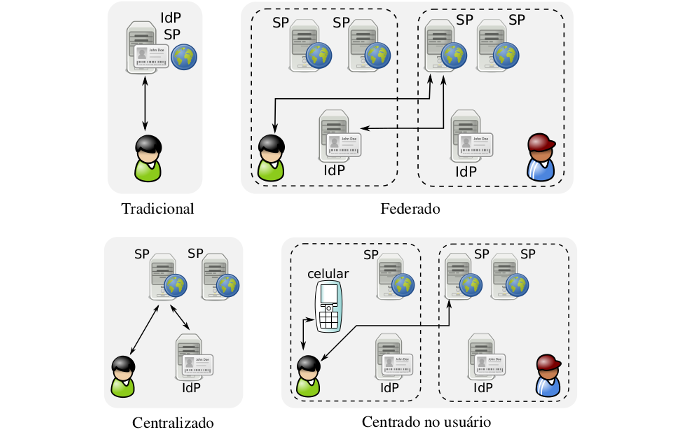
\includegraphics[width=.89\linewidth,fbox]{figs/Modelos_SGId.png}
  \caption{Classificação dos modelos de gerenciamento de identidade}
  \raggedright Fonte: Adaptado de %\citeonline{wangham:10}.
  \label{f_modelos_SGId}
\end{figure}



% ----------------------------------------------------------------------- %
\section{Exemplo de Tabela}
\label{ss_c2_exemplo-tabela}

%Uma tabela normalmente apresenta resultados quantitativos (números) e é usada para apresentar dados primários %\cite{oliveira:07}. Geralmente está presente em seções referentes aos resultados e do trabalho. Nada impede, porém, que uma tabela seja usada na fundamentação teórica.

A identificação da tabela é feita por uma legenda e por um título, separados por ponto, sendo que não se coloca o ponto final de parágrafo no final do título (conforme mostrado nos exemplos).

Quanto à formatação do seu conteúdo, podem ser usados espaçamento e fontes de letras com tamanhos menores que o do texto (não precisa seguir o mesmo padrão). Se o texto usa fonte 12, a tabela pode ser feita em fonte 11 ou 10.

Quando uma tabela for baseada em dados publicados em outro trabalho, a fonte de referência deve ser citada logo abaixo da tabela obedecendo às normas da ABNT4, indicando os autores do trabalho consultado e o ano da publicação do trabalho (entre parênteses),

\begin{table}[!htbp]
\begin{center}
\begin{footnotesize}
\caption{Exemplo de Tabela: Extração e Análise dos Dados - RSL 02}
\label{t_apendiceC-rsl}

\begin{tabular}{l|c|c|c|c|c|c|}
\cline{2-7}
 & \textbf{ACM} & \textbf{IEEExplore} & \multicolumn{1}{l|}{\textbf{ScienceDirect}} & \textbf{Scopus} & \textbf{Springer} & \textbf{Total de artigos} \\ \hline
\multicolumn{1}{|l|}{\textbf{Resultado da \textit{string} de busca}} & 24 & 26 & 9 & 49 & 154 & 262 \\ \hline
\multicolumn{1}{|l|}{\textbf{Trabalhos repetidos}} & 7 & 1 & 7 & 22 & 0 & 37 \\ \hline
\multicolumn{1}{|l|}{\textbf{Trabalhos removidos}} & 15 & 20 & 2 & 21 & 153 & 211 \\ \hline
\multicolumn{1}{|l|}{\textbf{Trabalhos pré-selecionados}} & 2 & 5 & 0 & 6 & 1 & 14 \\ \hline
\multicolumn{1}{|l|}{\textbf{Trabalhos aceitos}} & 1 & 1 & 0 & 2 & 0 & 4 \\ \hline
\end{tabular}

\end{footnotesize}
\end{center}
\raggedright Fonte: Elaborada pelo próprio autor.
\end{table}



% ----------------------------------------------------------------------- %
\section{Considerações}
\label{s_c2_consideracoes}

Texto das considerações do capítulo.

/% ----------------------------------------------------------------------- %
% Arquivo: cap3.tex
% ----------------------------------------------------------------------- %
\chapter{Trabalhos Relacionados}
\label{c_cap3}
Neste capítulo, será conduzido uma revisão sistemática com o objetivo de identificar estudos correlatos capazes de elucidar as questões do problema de pesquisa e enriquecer este trabalho. Duas indagações nortearam a busca pelos estudos relevantes, sendo importante ressaltar que os trabalhos encontrados não precisam ser idênticos, uma vez que os autores podem ter adotado abordagens distintas para solucionar o mesmo problema.

A estrutura deste capítulo é composta por três seções distintas. A Seção 3.1 descreve as perguntas de pesquisa, as estratégias de busca empregadas e os repositórios nos quais foram aplicadas. Na Seção 3.2, são apresentados os estudos relevantes que atendem aos critérios de inclusão e exclusão estabelecidos. Por fim, a Seção 3.3 realiza uma análise comparativa dos estudos selecionados.


%begin{itemize}
    %\item Definir critérios para a busca e para a análise dos trabalhos correlatos;
    
    %\item Efetuar a análise de cada trabalho com base nos critérios definidos;
    
    %\item Fazer uma análise comparativa (usualmente por meio de um quadro) entre os trabalhos, adicionando também a sua proposta.
%\end{itemize}

%Dessa forma, você poderá demonstrar como sua proposta se diferencia das demais, caracterizando a contribuição do trabalho.

%Dependendo da cobertura da revisão realizada e da atualidade dos trabalhos analisados, este capítulo pode ser denominado Estado da Arte. Contudo, essa decisão deve ser tomada em comum acordo com o seu orientador.

%É recomendado que a descrição do protocolo de busca e análise seja feita em um apêndice da dissertação, sendo que o nível de detalhamento a ser apresentando deve ser definido com o orientador.


% ----------------------------------------------------------------------- %
% ----------------------------------------------------------------------- %
\section{Definição dos critérios de busca}
\label{s_c3_trabalho-1}

%Você pode reservar uma seção para descrever cada trabalho selecionado. O título da seção é livre, mas deve permitir identificar o trabalho em análise.

Neste capítulo, foram pesquisados trabalhos que tenham como objetivo a análise de sistemas de armazenamento de energia associados a geração de energia solar. Além destes trabalhos, foi buscado trabalhos que tratem o gerenciamento de fluxo de potência nesse tipo de sistema de geração, bem como o desenvolvimento de ferramentas computacionais que auxiliem nessa análise.

Para conduzir a pesquisa, foram selecionados cinco repositórios como fontes para localizar os trabalhos relacionados. Os detalhes, incluindo os nomes e os endereços de acesso dos repositórios, estão apresentados na Tabela 1 abaixo:






% ----------------------------------------------------------------------- %
% ----------------------------------------------------------------------- %
\section{Trabalhos relacionados}
\label{s_c3_trabalho-2}

Descrição e crítica do trabalho relacionado.






% ----------------------------------------------------------------------- %
% ----------------------------------------------------------------------- %
\section{Comparação dos Trabalhos Relacionados}
\label{s_c3_comparacao}

%Nesta seção, apresente a análise comparativa dos trabalhos selecionados caracterizando-os em um quadro (conforme exemplificado no \autoref{q_c3-trabalhos}) e posicionando o seu trabalho em relação a eles (na última coluna). Dependendo da quantidade de trabalhos analisados, pode ser necessário elaborar mais de um quadro ou definir uma seção com página no formato paisagem.

%Mesmo que você ainda não tenha apresentado os resultados da sua dissertação no texto, isso conduzirá o restante da leitura, permitindo que você indique a contribuição de cada um dos trabalhos para a solução do problema de pesquisa da sua dissertação e evidencie a sua contribuição, e o diferencial do seu trabalho em relação aos demais. Isso deve ser feito por meio de um texto de discussão apoiado pelos dados apresentados no quadro. 

%Dica: utilizar o site ``\url{http://www.tablesgenerator.com/}'' para auxiliar na confecção dos quadros e tabelas.

 \begin{quadro}[!htbp]
 \caption{Comparação dos trabalhos relacionados} 
 \begin{center}
 \begin{footnotesize} 
 \label{q_c3-trabalhos} 
 
\resizebox{\textwidth}{!}{%
\begin{tabular}{|c|c|c|c|c|c|c|c|c|}
\hline
\rowcolor[HTML]{EFEFEF} 
{\color[HTML]{000000} \rotatebox[origin=c]{90}{\textbf{ Artigo }}} & {\color[HTML]{000000} \rotatebox[origin=c]{90}{\textbf{ Coluna 1 }}} & {\color[HTML]{000000} \rotatebox[origin=c]{90}{\textbf{ Coluna 2 }}} & {\color[HTML]{000000} \rotatebox[origin=c]{90}{\textbf{ Coluna 3 }}} & {\color[HTML]{000000} \rotatebox[origin=c]{90}{\textbf{ Coluna 4 }}} & {\color[HTML]{000000} \rotatebox[origin=c]{90}{\textbf{ Coluna 5 }}} & {\color[HTML]{000000} \rotatebox[origin=c]{90}{\textbf{ Coluna 6 }}} & {\color[HTML]{000000} \rotatebox[origin=c]{90}{\textbf{ Coluna 7 }}} & {\color[HTML]{000000} \rotatebox[origin=c]{90}{\textbf{ Coluna 8 }}} \\ \hline

\rowcolor[HTML]{C0C0C0} 
\textbf{\begin{tabular}[c]{@{}c@{}}MARTENS\\ (2010)\end{tabular}} & texto & texto & texto & \begin{tabular}[c]{@{}c@{}}quebra\\ linha\end{tabular} & texto & texto & texto & texto \\ \hline

\rowcolor[HTML]{EFEFEF} 
\textbf{\begin{tabular}[c]{@{}c@{}}EN-NASRY\\ E KETTANI \\ (2011)\end{tabular}} & texto & texto & texto & texto & texto & texto & texto & texto \\ \hline

\rowcolor[HTML]{C0C0C0} 
{\color[HTML]{000000} \textbf{\begin{tabular}[c]{@{}c@{}}BICAKCI\\ (2014)\end{tabular}}} & {\color[HTML]{000000} texto} & {\color[HTML]{000000} texto} & {\color[HTML]{000000} texto} & {\color[HTML]{000000} texto} & {\color[HTML]{000000} texto} & {\color[HTML]{000000} texto} & {\color[HTML]{000000} texto} & {\color[HTML]{000000} texto} \\ \hline

\rowcolor[HTML]{EFEFEF} 
\textbf{\begin{tabular}[c]{@{}c@{}}ESTE\\ TRABALHO\end{tabular}} & texto & texto & texto & texto & texto & texto & texto & texto \\ \hline

 \end{tabular}%
 } 
 \end{footnotesize}
 \end{center} 
 \raggedright Fonte: Elaborado pelo próprio autor. 
\end{quadro}


As publicações tratam disso e daquilo, suas contribuições são tal, mas não estão previstas tais coisas...

\begin{table}[]
\begin{tabular}{lllll}
 &  &  &  &  \\
 &  &  &  &  \\
 &  &  &  &  \\
 &  &  &  &  \\
 &  &  &  & 
\end{tabular}
\end{table}




% ----------------------------------------------------------------------- %
% ----------------------------------------------------------------------- %
\section{Considerações}
\label{s_c3_consideracoes}

Este capítulo pode ter uma última seção como esta denominada ``Considerações'' ou ``Discussão'' fazendo uma ligação entre a análise realizada sobre os trabalhos relacionados e o próximo capítulo, no qual você descreverá a sua contribuição.
% ----------------------------------------------------------------------- %
% Arquivo: cap4.tex
% ----------------------------------------------------------------------- %
\chapter{4  DESENVOLVIMENTO}
\label{c_cap4}

Neste capítulo, deve-se apresentar a contribuição da dissertação, ou seja, a solução desenvolvida para tratar o problema de pesquisa que motivou o trabalho. O título do capítulo é livre, podendo ser utilizado “Desenvolvimento”, ou outro que permita identificar mais claramente a solução desenvolvida.

Havendo necessidade, e em comum acordo com o orientador, este capítulo pode ser desdobrado em dois ou mais capítulos, se isso contribuir para melhorar a organização do documento. Por exemplo, se para um mesmo problema foram desenvolvidas duas soluções diferentes e, se para cada uma delas se justificar um capítulo exclusivo, existe liberdade para dividir este capítulo. O(s) capítulo(s) pode(m) ser organizado(s) de diferentes maneiras, ficando a cargo do autor e do seu orientador identificar aquela mais adequada à natureza do trabalho realizado. 

Em casos em que a dissertação possui uma contribuição complementar com um volume expressivo de informações que não são necessárias ao corpo da dissertação, essas informações podem ser colocadas em apêndices ou publicadas em um relatório técnico do Curso. Por exemplo, nos casos em que são desenvolvidos softwares que possuam manual de usuário, recomenda-se a sua publicação como relatório técnico, o qual pode ser citado pela dissertação. O mesmo se aplica ao projeto detalhado de sistemas de software e/ou de hardware desenvolvidos.



%_________________________
%_________________________
\section{Visão Geral e Premissas}
\label{s_c4_visao_geral}





%_________________________
\subsection{Detalhamento da Solução}
\label{ss_c4_detalhamento_mGov-BR}




%_________________________
\subsection{Requisitos Funcionais e Não Funcionais do Sistema Proposto}
\label{ss_c4_RF_RNF}

\begin{itemize}
    \item RF 01: requisito funcional 1;
    \item RF 02: requisito funcional 2;
    \begin{itemize}
        \item subitem do requisito funcional 2;        
    \end{itemize}    
\end{itemize}


\begin{itemize}
    \item RNF 01: requisito não funcional 1;
    \item RNF 02: requisito não funcional 2;
\end{itemize}


%_________________________
\subsection{Cenários de Uso}
\label{ss_c4_cenario-uso}

Para exemplificar a utilização da sistema XYZ proposto...


%_________________________
\subsubsection{Caso 01}
\label{sss_c4_caso-01}

Descrição do caso de uso 01;



%_________________________
\subsubsection{Caso 02}
\label{sss_c4_caso-02}

Descrição do caso de uso 02;



%_________________________
%_________________________
\section{Protótipo Desenvolvido}
\label{s_c4_prototipo}

Com o objetivo de avaliar a funcionalidade, usabilidade e desempenho da solução proposta, foi construído um protótipo em software, constituído de tal e tal coisa. Os atores são:

\begin{enumerate}
    \item Ator 1;
    \item Ator 2; e,
    \item Ator 3.
\end{enumerate}

Esta seção apresenta as ferramentas e tecnologias adotadas, bem como o detalhamento técnico da implementação do protótipo e a integração entre os atores.



%_________________________
\subsection{Ferramentas e Tecnologias Selecionadas}
\label{ss_c4_tecnologias}

Tecnologias seleciondas...




%_________________________
\subsection{Aplicativo X}
\label{ss_c4_aplicativoX}

Descrição do aplicativo X;



%_________________________
\section{Considerações}
\label{s_c4_consideracoes}

Este capítulo pode ter uma última seção como esta denominada ``Considerações'' ou ``Discussão'' discutindo o trabalho desenvolvido e fazendo uma ligação com o capítulo de análise de resultados.
% ----------------------------------------------------------------------- %
% Arquivo: cap.tex
% ----------------------------------------------------------------------- %
\chapter{Resultados}
\label{c_cap5}

Este capítulo é dedicado à apresentação e à discussão de resultados experimentais de modo a permitir que se possa avaliar a contribuição do trabalho, o alcance dos seus objetivos e a verificação das hipóteses de pesquisa.

Os experimentos realizados devem seguir um método científico (o qual deve ser descrito) e os seus resultados devem ser apresentados e discutidos pelo autor. Usualmente, utilizam-se tabelas, quadros e gráficos para apresentar os resultados experimentais, sendo que análise é feita de forma textual, conduzindo a discussão à verificação das hipóteses estabelecidas no início da pesquisa.




%_________________________
\section{Resultado dos Experimentos}
\label{s_c5_experimentos}

Esta seção descreve os resultados obtidos a partir de tal e tal...




%_________________________
\subsection{Experimento 01}
\label{ss_c5_CT01}

Os detalhes deste experimento são apresentados no \autoref{q_c5_CT01} de exemplo, que segue abaixo:

\


\begin{quadro}[!htbp]
 \caption{Caso de Teste 01 - exemplo do CT 01}
 \label{q_c5_CT01} 
 \begin{center}
 \begin{footnotesize} 

\begin{tabular}{|p{3.2cm}|p{13cm}|}
\hline
Tipo de teste & Funcional \\ \hline
Objetivo & texto \\ \hline
Pré-requisitos & texto \\ \hline
Dados de entrada & texto \\ \hline
Resultados esperados & texto \\ \hline
\end{tabular}
 
 \end{footnotesize}
 \end{center} 
 \raggedright Fonte: Elaborado pelo próprio autor. 
\end{quadro}


\noindent \textbf{Descrição do experimento 01:} aqui está toda a descrição do experimento...



%_________________________
\subsection{Experimento 02}
\label{ss_c5_CT02}

Descrição do experimento 02.




%_________________________
\subsection{Análise dos Experimentos}
\label{ss_c5_analise-experimentos}

Conclusão da análise feita...



%_________________________
\section{Avaliação da pesquisa de satisfação}
\label{s_c5_pesquisa}

Esta seção apresenta a avaliação da pesquisa de satisfação, realizada em um período de dez (10) dias, para o protótipo XYZ desenvolvido. O \autoref{apendice_f} apresenta o formulário de satisfação...., e o \autoref{apendice_g} apresenta as respostas coletadas...

A pesquisa foi respondida por vinte (20) profissionais de TI (tecnologia da informação) que trabalham em instituições governamentais e por treze (13) profissionais de TI que trabalham para empresas privadas, somando trinta e três (33) avaliações. 

%_________________________
\subsection{Avaliação dos Resultados}
\label{ss_c5_avaliacao-pesquisa}


\begin{enumerate}
    %Pesquisa de satisfação - experimentação 01
    \item Identificar tal e tal coisa.
    
    Descrição das análise...
\end{enumerate}
    
    
%_________________________
\section{Comparação com os trabalhos relacionados}
\label{s_c5_trab-relacionados}

Este trabalho, apresentou uma proposta XYZ, etc, etc, etc...


%_________________________
\section{Considerações}
\label{s_c5_consideracoes}

Este capítulo pode ter uma última seção como esta denominada ``Considerações'' ou ``Discussão'' consolidando a análise dos resultados.


% ---
% Finaliza a parte no bookmark do PDF
% para que se inicie o bookmark na raiz
% e adiciona espaço de parte no Sumário
% ---
\phantompart

% ---
% Conclusão
% ---
\chapter{Conclusão}
\label{c_conclusao}

Quais problemas este trabalho trata

O que foi feito até o momento (cap 2, 3 e 4)

Quais os próximos passos (com base no cap 4)

Resultados esperados... no modelo Univali está assim:

Este capítulo deve apresentar uma síntese sobre o trabalho desenvolvido, realizando uma análise a respeito do cumprimento dos objetivos estabelecidos e da verificação da hipótese de pesquisa inicial. Cada objetivo deve ser analisado, identificando-se o grau de atendimento (parcial ou integral), os problemas encontrados e as soluções adotadas, e justificando o porquê do não cumprimento integral (quando for o caso). Não devem ser apresentadas justificativas baseadas em dificuldades de natureza pessoal (ex. falta de tempo).


%_________________________
\section{Contribuição da Dissertação}
\label{c_conclusao-contribuicao}

Nesta seção, devem ser destacadas as principais contribuições do trabalho. Deve se identificar a relevância técnico-científica da pesquisa realizada, assim como os seus impactos social, ambiental e econômico (quando aplicável). Principalmente, deve-se ressaltar a contribuição do trabalho em relação ao estado da arte. Também podem ser identificados resultados alcançados quanto à publicações e patentes depositadas.


%_________________________
\section{Trabalhos Futuros}
\label{c_conclusao-trabalhos-futuros}

Esta seção deve identificar possíveis trabalhos que possam ser realizados a partir do desdobramento da pesquisa feita na dissertação. Procure discutir esses trabalhos como oportunidades de pesquisa que possam ser aproveitadas tanto por você como por outras pessoas.

Caso queira listar essas oportunidades, anteceda a lista por um parágrafo introdutório, como, por exemplo: “Ao longo do desenvolvimento deste trabalho, puderam ser identificadas algumas possibilidades de melhoria e de continuação a partir de futuras pesquisas, as quais incluem:”. Depois do parágrafo inicial, você pode listar as melhorias e continuações que podem ser feitas a partir do trabalho desenvolvido, mas procure comentar um pouco sobre cada proposta, mostrando que você já saberia como começar aquela nova pesquisa.



% ----------------------------------------------------------
% ELEMENTOS PÓS-TEXTUAIS
% ----------------------------------------------------------
\postextual

% ----------------------------------------------------------
% Referências bibliográficas
% ----------------------------------------------------------
%\bibliographystyle{abnt-alf}
\bibliography{11_referencias}

% ----------------------------------------------------------
% Glossário
% ----------------------------------------------------------
%
% Consulte o manual da classe abntex2 para orientações sobre o glossário.
%
%\glossary

% ----------------------------------------------------------
% Apêndices
% ----------------------------------------------------------

% ---
% Inicia os apêndices
% ---
\begin{apendicesenv}

% Imprime uma página indicando o início dos apêndices
%\partapendices
\setlength\afterchapskip{\lineskip}
% ----------------------------------------------------------------------- %
% Arquivo: 20_apendiceA.tex
% ----------------------------------------------------------------------- %
\chapter{Título do apêndice A}
\label{apendice_a}


Exemplo de inclusão de um documento em PDF:

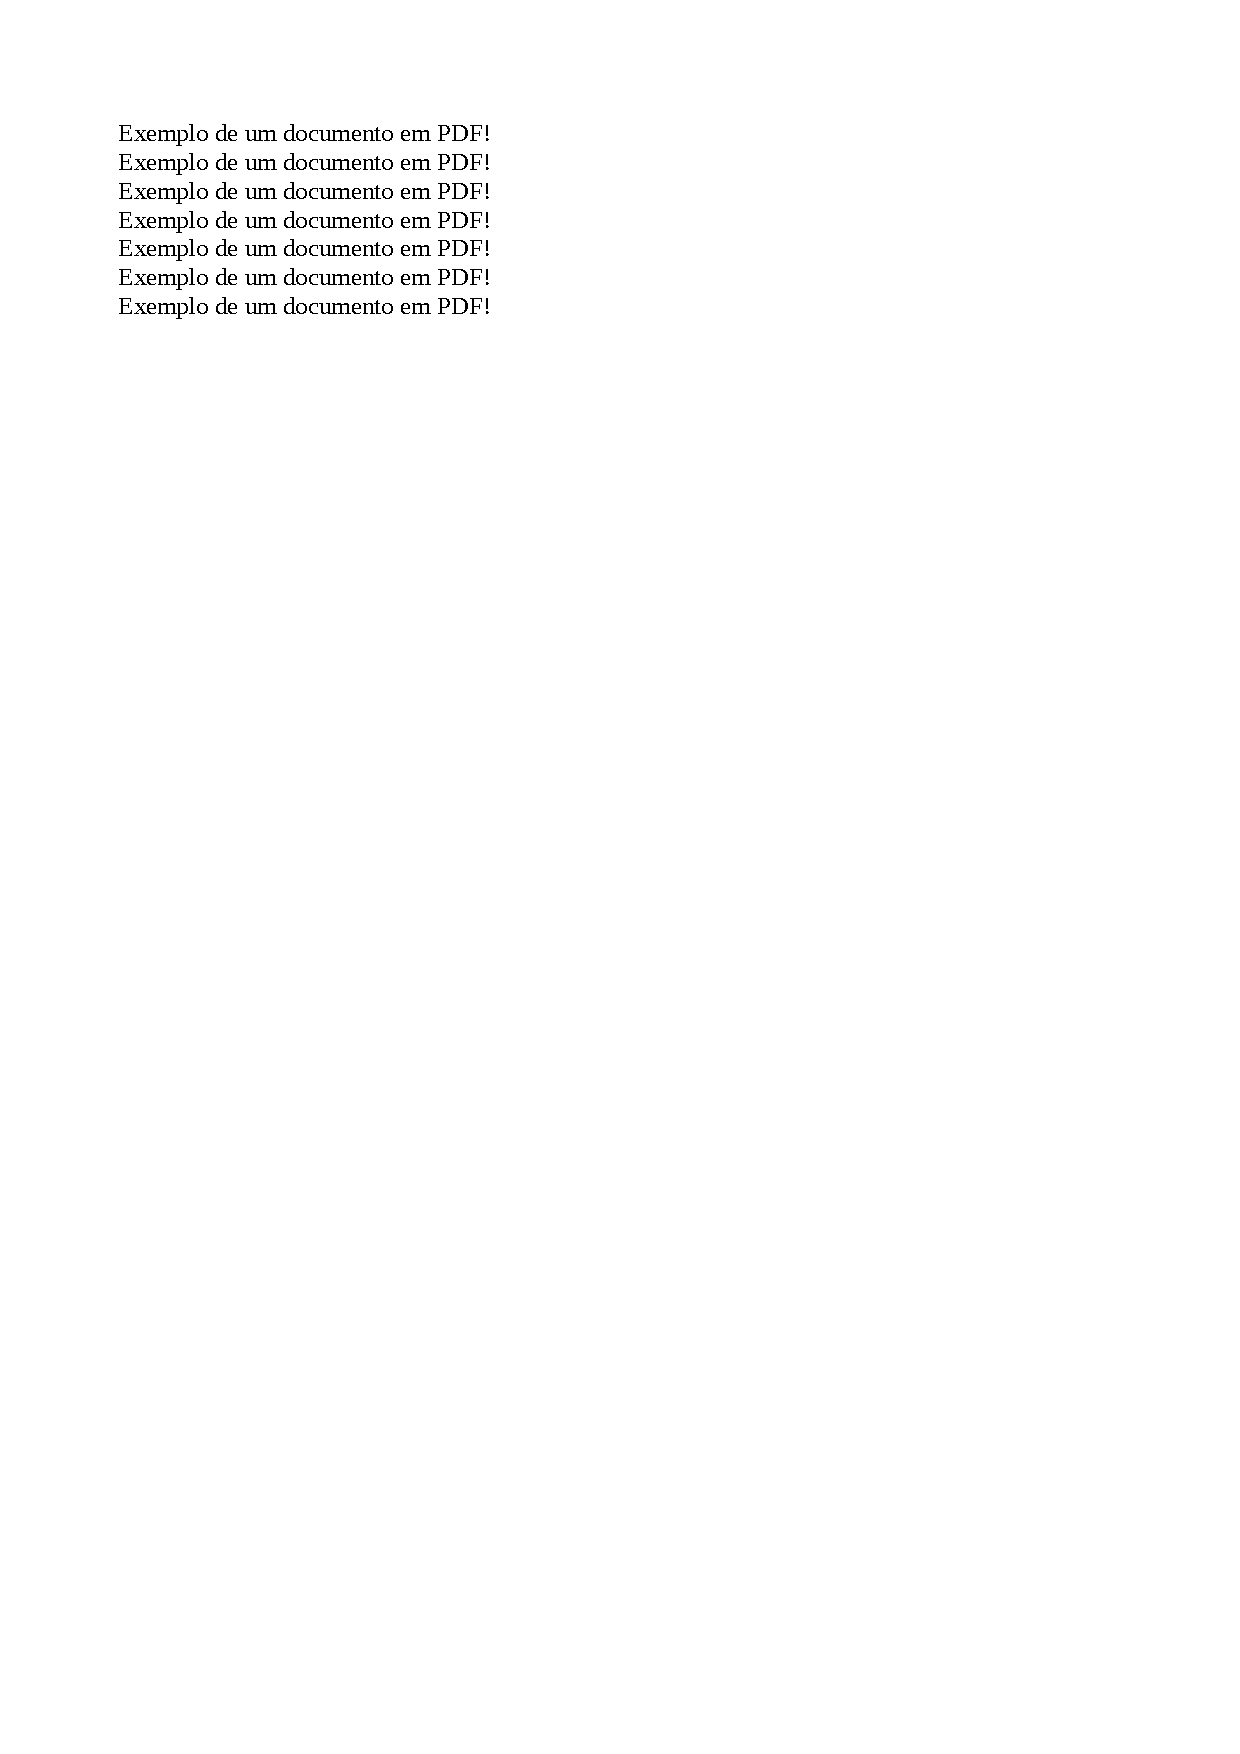
\includepdf[pages=1,scale=1]{pdf/exemplo.pdf}
% se o documento tiver mais páginas pode-se colocar assim: pages=1-2
% mesmo que o documento tenha mais de 2 páginas...
% ----------------------------------------------------------------------- %
% Arquivo: 21_apendiceB.tex
% ----------------------------------------------------------------------- %
\chapter{Título do apêndice B}
\label{apendice_b}



%_________________________
%_________________________
\section{Planejamento da Revisão Sistemática}
\label{s_apendiceB_planejamento}

\subsection{Questões de pesquisa}
\label{ss_apendiceB_objetivos}



%_________________________
\subsection{\textit{String} de Busca}
\label{ss_apendiceB_protocolo-busca}



%_________________________
\subsection{Identificação dos recursos}
\label{ss_apendiceB_id-recursos}




%_________________________
\subsection{Critérios de inclusão e exclusão}
\label{ss_apendiceB_criterios}





%_________________________
\subsection{Seleção dos artigos e extração dos dados}
\label{ss_apendiceB_extraction}





%_________________________
%_________________________
\section{Execução da Revisão Sistemática}
\label{s_apendiceB_execução}




%_________________________
\subsection{ACM}
\label{ss_apendiceB_acm}




%_________________________
\subsection{IEEExplore}
\label{ss_apendiceB_ieee}





%_________________________
\subsection{ScienceDirect}
\label{ss_apendiceB_sciencedirect}





%_________________________
\subsection{Scopus}
\label{ss_apendiceB_scopus}





%_________________________
\subsection{Springer}
\label{ss_apendiceB_springer}




%_________________________
%_________________________
\section{Resultados da Revisão Sistemática}
\label{s_apendiceB_resultado}




% ----------------------------------------------------------------------- %
% Arquivo: 22_apendiceC.tex
% ----------------------------------------------------------------------- %


\chapter{Título do apêndice C}
\label{apendice_c}


% ----------------------------------------------------------------------- %
% Arquivo: 23_apendiceD.tex
% ----------------------------------------------------------------------- %

\chapter{Título do apêndice D}
\label{apendice_d}


% ----------------------------------------------------------------------- %
% Arquivo: 24_apendiceE.tex
% ----------------------------------------------------------------------- %

\chapter{Título do apêndice E}
\label{apendice_e}


% ----------------------------------------------------------------------- %
% Arquivo: 25_apendiceF.tex
% ----------------------------------------------------------------------- %

\chapter{Título do apêndice F}
\label{apendice_f}



% ----------------------------------------------------------------------- %
% Arquivo: 26_apendiceG.tex
% ----------------------------------------------------------------------- %

\chapter{Título do apêndice G}
\label{apendice_g}



\end{apendicesenv}
% ---


% ----------------------------------------------------------
% Anexos
% ----------------------------------------------------------

% ---
% Inicia os anexos
% ---
%\begin{anexosenv}

% Imprime uma página indicando o início dos anexos
%\partanexos

%\setlength\afterchapskip{18pt}
%\include{30_anexoA}

%\end{anexosenv}

%---------------------------------------------------------------------
% INDICE REMISSIVO
%---------------------------------------------------------------------

\phantompart
\printindex

\end{document}